% AUTO-GENERATED by src/make_paper_assets.py -- do not edit.
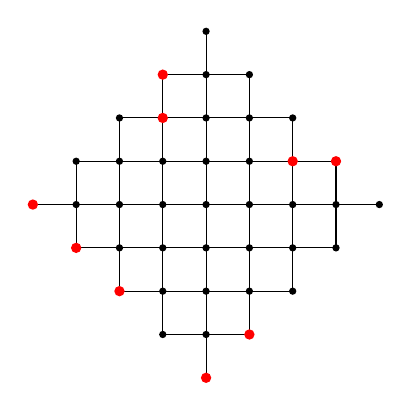
\begin{tikzpicture}[scale=0.55,every node/.style={inner sep=0}]
\draw (4,-4) -- (4,-4);
\draw (3,-3) -- (5,-3);
\draw (2,-2) -- (6,-2);
\draw (1,-1) -- (7,-1);
\draw (0,0) -- (8,0);
\draw (1,1) -- (7,1);
\draw (2,2) -- (6,2);
\draw (3,3) -- (5,3);
\draw (4,4) -- (4,4);
\draw (0,0) -- (0,0);
\draw (1,-1) -- (1,1);
\draw (2,-2) -- (2,2);
\draw (3,-3) -- (3,3);
\draw (4,-4) -- (4,4);
\draw (5,-3) -- (5,3);
\draw (6,-2) -- (6,2);
\draw (7,-1) -- (7,1);
\draw (8,0) -- (8,0);
\fill[black] (4,-4) circle (2.4pt);
\fill[black] (3,-3) circle (2.4pt);
\fill[black] (4,-3) circle (2.4pt);
\fill[black] (5,-3) circle (2.4pt);
\fill[black] (2,-2) circle (2.4pt);
\fill[black] (3,-2) circle (2.4pt);
\fill[black] (4,-2) circle (2.4pt);
\fill[black] (5,-2) circle (2.4pt);
\fill[black] (6,-2) circle (2.4pt);
\fill[black] (1,-1) circle (2.4pt);
\fill[black] (2,-1) circle (2.4pt);
\fill[black] (3,-1) circle (2.4pt);
\fill[black] (4,-1) circle (2.4pt);
\fill[black] (5,-1) circle (2.4pt);
\fill[black] (6,-1) circle (2.4pt);
\fill[black] (7,-1) circle (2.4pt);
\fill[black] (0,0) circle (2.4pt);
\fill[black] (1,0) circle (2.4pt);
\fill[black] (2,0) circle (2.4pt);
\fill[black] (3,0) circle (2.4pt);
\fill[black] (4,0) circle (2.4pt);
\fill[black] (5,0) circle (2.4pt);
\fill[black] (6,0) circle (2.4pt);
\fill[black] (7,0) circle (2.4pt);
\fill[black] (8,0) circle (2.4pt);
\fill[black] (1,1) circle (2.4pt);
\fill[black] (2,1) circle (2.4pt);
\fill[black] (3,1) circle (2.4pt);
\fill[black] (4,1) circle (2.4pt);
\fill[black] (5,1) circle (2.4pt);
\fill[black] (6,1) circle (2.4pt);
\fill[black] (7,1) circle (2.4pt);
\fill[black] (2,2) circle (2.4pt);
\fill[black] (3,2) circle (2.4pt);
\fill[black] (4,2) circle (2.4pt);
\fill[black] (5,2) circle (2.4pt);
\fill[black] (6,2) circle (2.4pt);
\fill[black] (3,3) circle (2.4pt);
\fill[black] (4,3) circle (2.4pt);
\fill[black] (5,3) circle (2.4pt);
\fill[black] (4,4) circle (2.4pt);
\fill[red] (4,-4) circle (3.4pt);
\fill[red] (5,-3) circle (3.4pt);
\fill[red] (2,-2) circle (3.4pt);
\fill[red] (1,-1) circle (3.4pt);
\fill[red] (0,0) circle (3.4pt);
\fill[red] (6,1) circle (3.4pt);
\fill[red] (7,1) circle (3.4pt);
\fill[red] (3,2) circle (3.4pt);
\fill[red] (3,3) circle (3.4pt);
\end{tikzpicture}
